%%%%
% Consiglio la visione dei seguenti tutorial:
% - https://www.youtube.com/watch?v=ihxSUsJB_14
% - https://www.youtube.com/watch?v=XTFWaV55uDo
%%%%
\documentclass[12pt,a4paper,openright,twoside]{book}
\usepackage[utf8]{inputenc}

%\newcommand{\thesislang}{italian} % decommentare in caso di tesi in italiano
\newcommand{\thesislang}{english} % commentare in caso di tesi in italiano
\usepackage{thesis-style}
% version
\newcommand{\versionmajor}{0}
\newcommand{\versionminor}{1}
\newcommand{\versionpatch}{2}
\newcommand{\version}{\versionmajor.\versionminor.\versionpatch}
\typeout{Document version: \version}

\begin{document}
	
\frontmatter

% ! TeX root = thesis-main.tex
\title{Title}
\author{Candidate Name Here}
\date{\today}

\newgeometry{margin=0.8in}
\begin{titlepage}
	\begin{center}
		% \vspace*{0.2cm}
		
		\large
		\textbf{ALMA MATER STUDIORUM -- UNIVERSITÀ DI BOLOGNA \\ CAMPUS DI CESENA}
		\\
		\noindent\hrulefill
		\vspace{0.4cm}
		
		\Large
		Scuola di Ingegneria e Architettura \\
		Corso di Laurea (Magistrale) in Ingegneria e Scienze Informatiche
		
		\Huge
		\vspace{4cm}
		\textbf{
			Fair-by-design matching algorithm
		}
		
		\large
		\vspace{1cm}
		Tesi di laurea in 
		\\
		\textsc{(Intelligent System Engineering)}
		
		\vspace{5.5cm}
		\begin{minipage}[t]{0.64\textwidth}
			\begin{flushleft}
				\textit{Relatore} 
				\\ 
				(\textbf{Prof.} $\mid$ \textbf{Dott.}) \textbf{Nome Cognome}
				\\
				\vspace{0.4cm}
				\textit{Correlatore} 
				\\
				(\textbf{Ing.})? \textbf{Dott.} \textbf{Nome Cognome}
			\end{flushleft}
		\end{minipage}
		\begin{minipage}[t]{0.34\textwidth}
			\begin{flushright}
				\textit{Candidato} 
				\\ 
				\textbf{Antonio Iannotta}
			\end{flushright}
		\end{minipage}\\
		
		\vfill
		\noindent\hrulefill
		\vspace{0.3cm}
		\Large
		
		%(N-Esima) Sessione di Laurea
		II Sessione di Laurea
		\\
		Anno Accademico 2022-2023
	\end{center}
\end{titlepage}
\restoregeometry


\begin{abstract}	
Artificial Intelligence (AI) has revolutionized many sectors, including matching, by providing automated solutions for resource, opportunity, or information associations. However, the widespread use of matching algorithms in AI can also lead to potential discrimination, amplifying existing inequalities in society. This thesis focuses on the development of fair-by-design algorithms for matching in the field of artificial intelligence to ensure ethical, transparent, and non-discriminatory association decisions.

Throughout the research, various fundamental aspects of matching in the context of AI and the associated ethical implications are examined. The main challenges related to discrimination, fairness, and transparency in the matching process are identified. Subsequently, the current approaches and methodologies available for developing fair-by-design algorithms are presented and analyzed.

The thesis proposes a novel approach to matching that integrates fairness and discrimination criteria within the algorithmic process. Different fairness and discrimination metrics are explored to assess the impact of matching algorithms on the distribution of opportunities and equitable treatment of different user categories.

The implementation of fair-by-design algorithms for matching is evaluated through a series of case studies, where the performance of the proposed algorithms is analyzed and compared to conventional solutions. The results demonstrate that fair-by-design algorithms can significantly reduce disparities and discrimination compared to traditional matching methods.

Finally, guidelines are proposed for developers and stakeholders interested in matching in the field of AI, aiming to promote the adoption of fair-by-design algorithms and encourage ethical and responsible use of artificial intelligence.
\end{abstract}

\begin{dedication} % this is optional
Optional. Max a few lines.
\end{dedication}

\begin{acknowledgements} % this is optional
Optional. Max 1 page.
\end{acknowledgements}

%----------------------------------------------------------------------------------------
\tableofcontents   
\listoffigures     % (optional) comment if empty
\lstlistoflistings % (optional) comment if empty
%----------------------------------------------------------------------------------------

\mainmatter

%----------------------------------------------------------------------------------------
\chapter{\introductionname}
\label{chap:introduction}
%----------------------------------------------------------------------------------------

%Write introduction here.

\section{Background}
In recent years, the use of artificial intelligence (AI) algorithms for matching has become prevalent in various domains, including job recruitment, dating platforms, and resource allocation. These algorithms aim to automate the process of connecting entities based on specific criteria, optimizing compatibility, or minimizing distance. However, there is growing concern about the potential biases and discriminatory outcomes that may arise from the use of such algorithms. It is crucial to address these concerns and develop fair-by-design algorithms that ensure fairness and mitigate discrimination in the matching process.

\section{Fairness in AI}
Fairness is a central concept when designing and implementing AI systems. It involves treating individuals fairly and avoiding unjust or biased outcomes based on characteristics such as race, gender, or socioeconomic status. In the context of matching algorithms, fairness aims to ensure that the allocation of resources or opportunities is equitable and does not favor or discriminate against certain individuals or groups.

\subsection{Types of Fairness}
There are various notions of fairness that can be considered when developing fair-by-design algorithms for matching. Some commonly discussed types include:

\begin{itemize}
    \item \textbf{Statistical Fairness}: This refers to ensuring that the outcomes of the matching process are statistically equitable across different groups. For example, an algorithm should not consistently favor one group over another in terms of resource allocation.
    \item \textbf{Individual Fairness}: Individual fairness focuses on treating similar individuals similarly. It aims to ensure that individuals who have similar characteristics or qualifications receive similar opportunities or resources.
    \item \textbf{Group Fairness}: Group fairness is concerned with ensuring that certain predefined groups receive equitable treatment in the matching process. This can involve equal representation or distribution of opportunities among different groups.
\end{itemize}

\section{Matching Algorithms}
Matching algorithms play a crucial role in various applications of AI. They involve the assignment of resources, individuals, or opportunities to optimize specific objectives. Common types of matching algorithms include the stable marriage algorithm, bipartite graph matching, and recommendation systems. These algorithms often rely on historical data or user preferences to make matches, which can introduce biases and perpetuate existing societal inequalities.

\subsection{Challenges in Fairness for Matching Algorithms}
Applying fairness to matching algorithms introduces unique challenges. One key challenge is the trade-off between fairness and optimizing matching outcomes. Striking a balance between these objectives requires careful algorithm design and considerations of fairness metrics. Additionally, addressing potential biases in the data used by the algorithms is crucial for achieving fair outcomes.

\section{Impact of Fairness in AI Systems on Society}
The fairness of AI systems, including matching algorithms, has a profound impact on society. Biased or discriminatory outcomes in matching can perpetuate and reinforce existing inequalities. For example, biased job matching algorithms may favor certain demographic groups, resulting in limited opportunities for others. Unfairness in important domains such as education, employment, or housing can have long-lasting effects on individuals and communities. It is essential to develop fair-by-design algorithms to mitigate these negative consequences and promote equal opportunities.

\subsection{Ethical Considerations}
Developing fair-by-design algorithms requires careful consideration of ethical implications. Fairness should not be pursued at the expense of other ethical principles such as privacy, transparency, or accountability. Striking the right balance between fairness and other considerations is vital to ensure the responsible implementation of matching algorithms.

\section{Thesis Objectives}
This thesis aims to explore the implementation of fair-by-design algorithms for matching and their impact on ensuring fairness in AI systems. The specific objectives are:

\begin{itemize}
    \item Investigate different fairness metrics and criteria applicable to matching algorithms.
    \item Develop novel fair-by-design algorithms for matching that balance fairness and optimization objectives.
    \item Assess the performance and effectiveness of the proposed fair-by-design algorithms through empirical evaluations and case studies.
    \item Analyze the societal impact of fair matching algorithms and the potential benefits of integrating fairness into AI systems.
\end{itemize}


%
\paragraph{Thesis Structure.} % Optional paragraph title
%

(This is optional an optional paragraph.)
%
Accordingly, the reminder of this thesis is structures as follows.
%
\Cref{chap:background} discusses (briefly describe the content of \cref{chap:background}).
%
Describe other chapters here in a similar way.
%
Finally, \Cref{chap:conclusions} concludes this thesis by summarising its main contribution.

%----------------------------------------------------------------------------------------
\chapter{State of the Art} % or Background
\label{chap:background}
%----------------------------------------------------------------------------------------

%Write background here.

%This section is likely to contain a lot of citations.
%
%For instance in \cite{AnzengruberSocInfo2013} the authors propose a novel means for tackling with the problem of preventing bad things from happening.

%----------------------------------------------------------------------------------------
\chapter{Design} % possible chapter for Projects
\label{chap:design}
%----------------------------------------------------------------------------------------

Write design here.

\begin{figure}
	\centering
	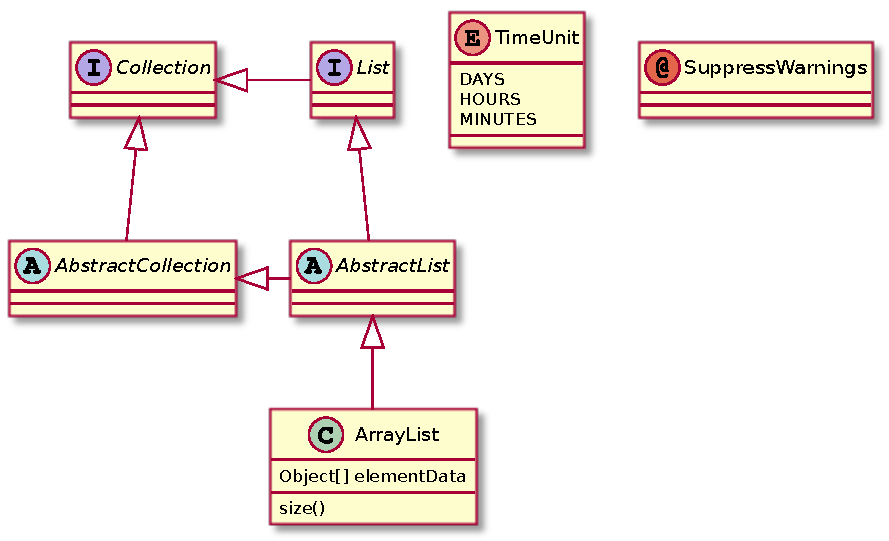
\includegraphics[width=0.5\linewidth]{figures/classes.pdf}
	\caption{A class diagram created with PlantUML}
	\label{fig:classes}
\end{figure}

You may want to reference images in your thesis.
%
In this case, you are encouraged to make them \emph{floating}, and reference them by means of labels.
%
For instance, in \Cref{fig:classes}, we describe a class diagram produced by means of \href{http://plantuml.com}{PlantUML}.

%----------------------------------------------------------------------------------------
\chapter{Implementation} % possible chapter for Projects
\label{chap:implementation}
%----------------------------------------------------------------------------------------

Write implementation here.

\lstinputlisting[
	float,
	language=Java,
	caption={My very first program in Java},
	label={lst:helloworld},
]{listings/HelloWorld.java}

You may need to reference listings in your thesis.
%
In this case, you are encouraged to make them \emph{floating}, and reference them by means of labels.
%
For instance, in \Cref{lst:helloworld}, we describe an hello world program in Java.

%----------------------------------------------------------------------------------------
\chapter{Validation} % possible chapter for Projects
\label{chap:validation}
%----------------------------------------------------------------------------------------

Write implementation here

%----------------------------------------------------------------------------------------
\chapter{\conclusionsname}
\label{chap:conclusions}
%----------------------------------------------------------------------------------------

Write conclusions here.


%----------------------------------------------------------------------------------------
% BIBLIOGRAPHY
%----------------------------------------------------------------------------------------

\nocite{*} % uncomment this to show all the reference in the .bib file
\bibliographystyle{plain}
\bibliography{bibliography}


\end{document}